\documentclass[11pt,letterpaper]{article}
\usepackage[T1]{fontenc}
\usepackage[utf8]{inputenc}
\usepackage{lmodern}
\usepackage[margin=0.85in]{geometry}
\usepackage{amsmath,amssymb}
\usepackage{graphicx,booktabs,array}
\usepackage{xcolor}
\usepackage{float,caption}
\usepackage{fancyhdr}
\usepackage{listings}
\usepackage{hyperref}
\definecolor{navy}{HTML}{183B56}
\definecolor{teal}{HTML}{116466}
\definecolor{codegray}{HTML}{F5F7F9}
\hypersetup{colorlinks=true,linkcolor=navy,urlcolor=teal,citecolor=navy,
  pdftitle={FRE7241 Homework 1: Portfolio Allocation and ETF Alpha},
  pdfauthor={Panagiotis Housos}}
\pagestyle{fancy}
\fancyhf{}
\fancyhead[L]{\small FRE7241 \quad Homework 1}
\fancyhead[R]{\small Panagiotis Housos}
\fancyfoot[C]{\thepage}
\setlength{\headheight}{14pt}
\setlength{\parindent}{0pt}
\setlength{\parskip}{0.55em}
\setlength{\emergencystretch}{2em}
\clubpenalty=10000
\widowpenalty=10000
\renewcommand{\arraystretch}{1.12}
\captionsetup{font=small,labelfont=bf}
\lstdefinestyle{rcode}{language=R,basicstyle=\ttfamily\scriptsize,
  keywordstyle=\color{navy},commentstyle=\color{teal},
  stringstyle=\color{black},numbers=left,numberstyle=\tiny\color{gray},
  numbersep=7pt,backgroundcolor=\color{codegray},frame=single,
  rulecolor=\color{gray!25},breaklines=true,breakatwhitespace=false,
  columns=fullflexible,keepspaces=true,showstringspaces=false,
  tabsize=2,xleftmargin=12pt,framexleftmargin=10pt}
\lstset{style=rcode}
\newcommand{\wideinput}[3]{%
  \begin{table}[H]\centering
  \caption{#2}\label{#3}
  \resizebox{\linewidth}{!}{\input{tables/#1}}
  \end{table}}
\newcommand{\smallinput}[3]{%
  \begin{table}[H]\centering
  \caption{#2}\label{#3}
  {\small\input{tables/#1}}
  \end{table}}
% Generated by report/export_results.R; do not edit numerical results.
\newcommand{\HWPriceRows}{5962}
\newcommand{\HWReturnRows}{5028}
\newcommand{\HWBootSamples}{1000}
\newcommand{\HWCapmYears}{21}
\newcommand{\HWPriceStart}{2002-07-26}
\newcommand{\HWPriceEnd}{2026-04-07}
\newcommand{\HWReturnStart}{2006-04-11}
\newcommand{\HWReturnEnd}{2026-04-07}
\newcommand{\HWTenYearWeight}{0.4543241}
\newcommand{\HWEqualRiskRatio}{6.934682}
\newcommand{\HWOptimalRiskRatio}{7.043107}
\newcommand{\HWAlphaCorrelation}{-0.239298}
\newcommand{\HWAlphaSignSameCount}{4}
\newcommand{\HWAlphaSignChangedCount}{4}
\newcommand{\HWFirstWindowRows}{183}
\newcommand{\HWLastWindowRows}{66}
\newcommand{\HWLastYearActualRows}{65}
\newcommand{\HWLastWindowStart}{2025-12-31}
\newcommand{\HWLastWindowEnd}{2026-04-07}
\newcommand{\HWLastTopETF}{USO}
\newcommand{\HWLastTopAlpha}{9.9429}
\newcommand{\HWTenYearAvailableBlocks}{3443}
\newcommand{\HWTenYearOverlapPct}{93.901}
\newcommand{\HWTenYearMeanOverlapPct}{56.481}
\newcommand{\HWTenYearDisjointBlocks}{2}


\begin{document}
\hypersetup{pageanchor=false}
\begin{titlepage}
\vspace*{0.6in}
{\color{teal}\large NYU Tandon School of Engineering\par}
\vspace{0.25in}
{\color{navy}\LARGE Algorithmic Portfolio Management\par}
\vspace{0.15in}
{\large FRE7241 \quad Homework 1\par}
\vspace{0.65in}
{\color{navy}\Huge Portfolio Allocation\\[0.12in]and ETF Alpha\par}
\vspace{0.3in}
{\Large Methods, results, and interpretation\par}
\vspace{0.65in}
{\Large Panagiotis Housos\par}
\vspace{0.12in}
{\large October 29, 2026\par}
\vfill
\begin{minipage}{0.94\textwidth}
\textbf{What this report contains.} Solutions to all eight questions, the
historical bootstrap and optimization methods, complete annual alpha and
ranking matrices, both requested plots, all annual CAPM tables, the full
submitted R code, the execution output, and independent verification.

The approximately ten-year bootstrap selects a VTI weight of
$\HWTenYearWeight$. The annual ETF analysis produces an $8\times21$ alpha
matrix. All ten independent numerical and artifact checks pass.
\end{minipage}
\end{titlepage}
\pagenumbering{roman}
\hypersetup{pageanchor=true}

\section*{Abstract}
This homework studies two historical portfolio questions using the supplied
\texttt{rutils::etfenv} data. First, a paired historical block bootstrap
constructs 1,000 cumulative VTI and IEF log-return scenarios at each investment
horizon. A bounded scalar optimization maximizes the mean-to-standard-deviation
ratio of the assignment's weighted cumulative log-return measure. The
approximately ten-year optimal stock allocation is 45.43\%, while allocations
across the five requested horizons range from 35.97\% to 45.88\% and are not
monotonic. Second, yearly endpoint intervals are used to estimate CAPM-style
statistics for eight ETFs against VTI. The report presents the full annualized
alpha and ranking matrices and a 2008--2009 alpha scatterplot. It distinguishes
the package's annualization convention from realized returns, documents shared
interval boundaries and partial years, and records the robust-regression
warning. Independent moment-based optimization and ordinary least-squares
calculations verify the numerical results.

\tableofcontents
\clearpage
\pagenumbering{arabic}

\section{Data, conventions, and reproducibility}
\label{sec:data}
The solution follows the course's bootstrap, R functional-programming, and
CAPM examples~\cite{univariate,functions,dates,data}. The executable submission
is \texttt{Panagiotis\_Housos\_hw1.R}. Its values are computed from the data;
the professor's example output is used as a diagnostic, rather than inserted
into the calculations.

Part I selects VTI and IEF prices, removes rows with missing prices, extracts
a numeric matrix, and takes logarithms. The resulting
paired sample contains \HWPriceRows{} observations from
\texttt{\HWPriceStart} through \texttt{\HWPriceEnd}. Part II selects VTI, IEF,
VNQ, USO, XLY, XLP, XLE, XLF, and XLK, applies the assigned
\texttt{na.locf()} and \texttt{na.omit()} preprocessing, and contains
\HWReturnRows{} daily observations from \texttt{\HWReturnStart} through
\texttt{\HWReturnEnd}.

The supplied return series contains \emph{log returns}, as confirmed against
differences of log prices. This matters for interpreting both the portfolio
metric and the regression outputs.

Two indexing conventions follow the assignment and lecture examples:
\begin{itemize}
\item A holding block of $h$ price observations starts at row $s$ and ends at
row $s+h-1$, spanning $h-1$ daily return intervals. The code samples from all
$N-h+1$ valid starting rows, including the last possible block.
\item A CAPM interval includes both neighboring endpoint rows. Consequently,
adjacent intervals share one boundary observation. These are the assignment's
endpoint windows, rather than strictly disjoint calendar-year samples.
\end{itemize}

All simulations use the specified seed 1121, the Mersenne--Twister generator,
and rejection sampling. The repository records package versions, GitHub
source commits, the R session, input-data fingerprints, complete scenario
exports, and verification results. The analysis is historical and in sample;
it does not evaluate an allocation or ranking strategy on a held-out period.

\section{Part I: optimal stock and bond allocations}
\subsection{I.1: bootstrap scenarios and portfolio wealth measure}
Let $L_{t,a}=\log P_{t,a}$ be asset $a$'s log price. For bootstrap draw
$b=1,\ldots,B$, sample a starting index independently with replacement:
\begin{equation}
s_b\sim\operatorname{Uniform}\{1,\ldots,N-h+1\},\qquad B=1000.
\end{equation}
The paired cumulative log-return scenario is
\begin{equation}
R_{a,b}^{(h)}=L_{s_b+h-1,a}-L_{s_b,a}.
\label{eq:bootstrap}
\end{equation}
The same historical dates are used for both assets, preserving their joint
holding-period behavior. The transposed differences form a $2\times1000$
matrix, with assets in rows and scenarios in columns. For the initial
approximately ten-year calculation, $h=10\times252=2520$ price observations.

\wideinput{ten_year_returns_first5.tex}{The first five paired approximately
ten-year bootstrap scenarios. Entries are cumulative log returns.}{tab:tenreturns}

For stock weight $w$, the assignment defines
\begin{equation}
W_b(w)=wR_{\mathrm{VTI},b}^{(h)}+(1-w)R_{\mathrm{IEF},b}^{(h)}.
\label{eq:wealth}
\end{equation}
The implementation calculates this with a matrix product and uses
\texttt{drop()} to obtain a length-1000 vector. Table~\ref{tab:equalwealth}
shows the first five values at $w=0.5$.

\smallinput{wealth_first5.tex}{The first five portfolio-metric values at the
50/50 allocation, using the scenarios in Table~\ref{tab:tenreturns}.}{tab:equalwealth}

\textbf{Interpretation.} Although the assignment calls $W$ ``wealth,'' it is a
weighted cumulative log-return metric. If the initial dollar allocation were
held without rebalancing, terminal gross wealth per initial dollar would be
\begin{equation}
G_b(w)=w\exp(R_{\mathrm{VTI},b}^{(h)})
       +(1-w)\exp(R_{\mathrm{IEF},b}^{(h)}),
\end{equation}
and $\log G_b(w)$ generally differs from $W_b(w)$. The submitted solution
optimizes the measure requested in the assignment.

\subsection{I.2: risk adjustment and bounded optimization}
For a given scenario matrix, define
\begin{equation}
J_h(w)=\frac{\overline{W(w)}}{s_{W(w)}},\qquad
w_h^\star=\arg\min_{0\leq w\leq1}\{-J_h(w)\}.
\label{eq:objective}
\end{equation}
The function \texttt{riskretfun(retm, weightv)} returns the negative ratio;
\texttt{optimize()} minimizes it over \texttt{c(0,1)}. The bounds represent a
fully invested, long-only allocation with weights $w$ and $1-w$.

For the 50/50 approximately ten-year sample, the portfolio metric has mean
$0.7109867$ and sample standard deviation $0.1025262$. Its mean/SD ratio is
$\HWEqualRiskRatio$, so the objective is its negative. Optimization gives
\begin{equation}
\boxed{w_{\mathrm{VTI}}^\star=\HWTenYearWeight,
\qquad w_{\mathrm{IEF}}^\star=1-\HWTenYearWeight.}
\end{equation}
Thus the optimized allocation is approximately 45.43\% VTI and 54.57\% IEF,
with optimized ratio $\HWOptimalRiskRatio$.

This ratio describes the cumulative horizon metric across sampled windows.
It is not an annualized daily Sharpe ratio and does not subtract a risk-free
return. Independent inverse-covariance calculations agree with the numerical
optimum within the optimizer's default tolerance.

\subsection{I.3: allocations at the five requested horizons}
The requested horizons are generated from the sample size:
\begin{equation}
\boldsymbol h=\operatorname{round}\!\left(N(0.1,0.2,0.3,0.4,0.5)\right)
=(596,1192,1789,2385,2981).
\end{equation}
A named list stores one $2\times1000$ paired return matrix per horizon.
An \texttt{sapply()} loop calls \texttt{optimize()} separately for each matrix
and returns a named vector of optimal VTI allocations.

\wideinput{horizon_summary.tex}{Optimized allocations and portfolio-metric
summary statistics across the five holding blocks. Trading years use
$(h-1)/252$; metrics are cumulative log-return quantities.}{tab:horizons}

\begin{figure}[H]\centering
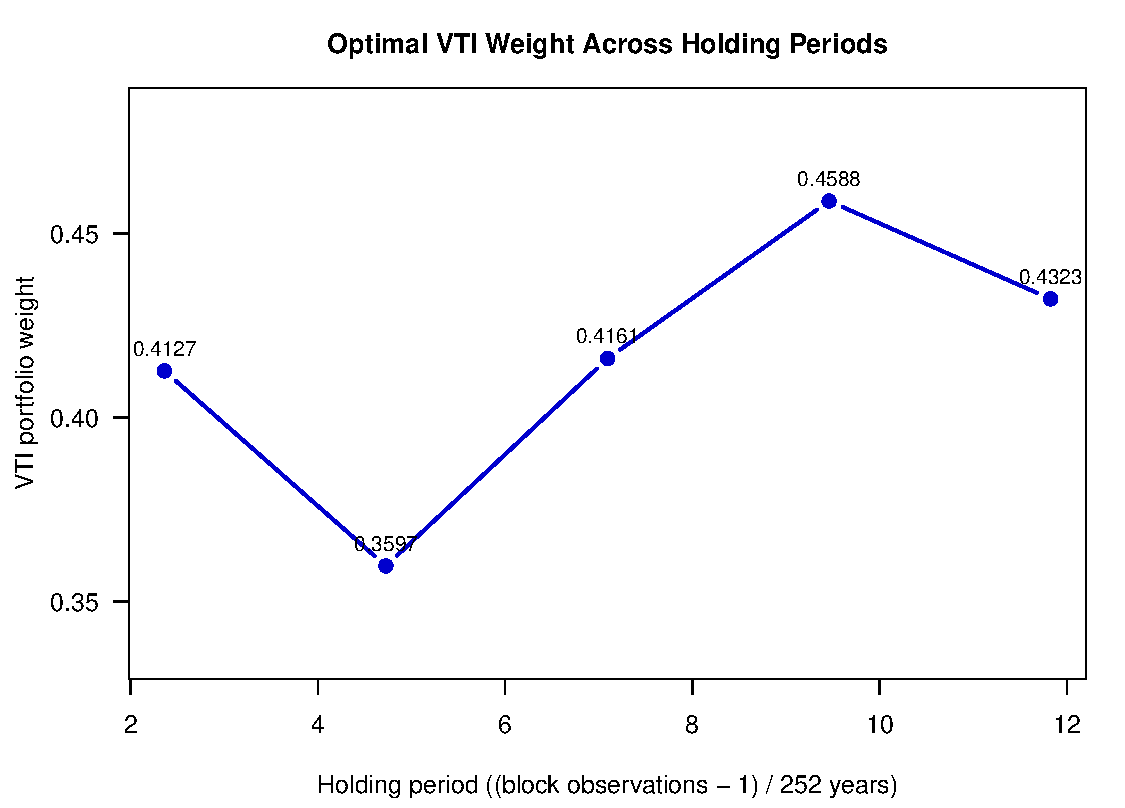
\includegraphics[width=0.92\linewidth]{figures/optimal_weights_by_horizon.pdf}
\caption{Optimal VTI allocations across the five requested holding blocks.
The connecting line describes these five historical estimates.}
\label{fig:weights}
\end{figure}

\textbf{Commentary.} The stock weights are not monotonic in the holding
period. They fall from 41.27\% to 35.97\%, rise to 45.88\%, then fall to
43.23\% at the longest horizon. Therefore the results do not support an
unqualified claim that optimal stock exposure always increases with the
investment horizon. The asset-return correlation is least negative in the
shortest-horizon sample, but this descriptive pattern alone does not establish
why an optimal weight changes.

The portfolio variance is
\begin{equation}
\operatorname{Var}(W)=w^2\sigma_V^2+(1-w)^2\sigma_I^2
     +2w(1-w)\operatorname{Cov}(R_V,R_I).
\end{equation}
Both expected cumulative returns and their joint dispersion change with the
horizon, so the allocation depends on more than asset correlation.

\subsection{I.4: portfolio distributions and historical interpretation}
An \texttt{lapply()} loop over the named scenario list combines each matrix
with its matching optimal weight. It produces five named length-1000 vectors.
The first five shortest-horizon scenarios and portfolio values are recorded
in Appendix~\ref{app:additional}.

\begin{figure}[H]\centering
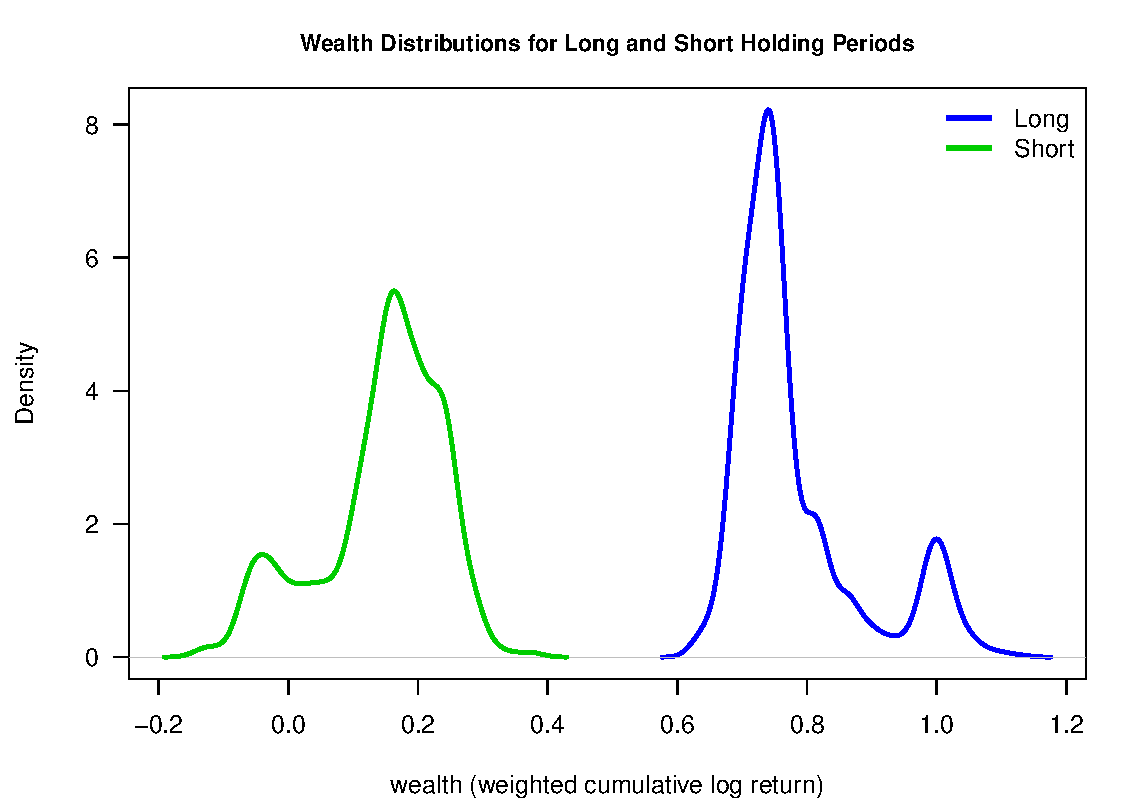
\includegraphics[width=0.96\linewidth]{figures/portf_wealth_longshort.pdf}
\caption{Kernel-density estimates of the optimized portfolio metric at the
longest (blue) and shortest (green) holding blocks. The horizontal axis uses
the assignment's cumulative log-return ``wealth'' convention.}
\label{fig:wealth}
\end{figure}

The longest-horizon distribution lies farther to the right. Its sample mean
is approximately $0.78049$, compared with $0.14457$ for the shortest horizon.
The corresponding standard deviations are approximately $0.09988$ and
$0.09493$. In particular, the rightward shift is not evidence that absolute
dispersion is smaller at the longest horizon. The shortest sample has 11.8\%
negative portfolio-metric values, while the longest sample has none.

These are frequencies among historical windows, not established future loss
probabilities. Bootstrap draws are independent conditional on the fixed
empirical dataset, but the underlying historical blocks overlap and may be
sampled repeatedly. One thousand draws therefore do not represent one
thousand newly observed independent market episodes. The overlap diagnostics
in Appendix~\ref{app:additional} quantify this distinction without treating
them as an estimate of effective sample size. The favorable historical
sample, changing market regimes, and the absence of an out-of-sample test
limit any extrapolation of these optimized allocations.

\clearpage
\section{Part II: annual ETF alpha and rankings}
\subsection{II.1: yearly endpoint intervals and CAPM tables}
\texttt{rutils::calc\_endpoints(retp, interval = "years")} supplies the year-end
row positions, with initial zero and the final observation included. There
are \HWCapmYears{} intervals, labeled by their ending years 2006--2026.
Following the assignment's example, interval $i$ uses rows
\begin{equation}
\max(1,e_i),\ldots,e_{i+1}.
\end{equation}
Thus the final interval begins on \texttt{\HWLastWindowStart}, includes the
previous year's boundary observation, and ends on
\texttt{\HWLastWindowEnd}. The first interval has \HWFirstWindowRows{}
observations and the last has \HWLastWindowRows{} observations; the final
interval contains \HWLastYearActualRows{} observations actually dated 2026.
The first and last years are partial. All window dates and row counts appear
in Appendix~\ref{app:additional}.

For comparison asset $a$ in a given interval, the ordinary regression is
\begin{equation}
r_{a,t}=\alpha_a+\beta_a r_{\mathrm{VTI},t}+\varepsilon_{a,t},
\label{eq:capm}
\end{equation}
where the supplied $r$ are daily log returns and the assigned risk-free rate
is zero. \texttt{table.CAPM()} compares the eight non-benchmark ETFs against
VTI and calculates the requested summary table. Column names such as
\texttt{IEF to VTI} are simplified to the ETF ticker, and the list is named
with the interval-ending years.

\wideinput{capm_first_year.tex}{Complete CAPM table for the first interval,
2006. The remaining annual tables are in Appendix~\ref{app:capm}. Values
retain the package's four-decimal reporting convention.}{tab:capmfirst}

The package reports ordinary and robust coefficients, conditional up/down
betas, correlations, and benchmark-relative performance measures. During the
2012 VNQ \texttt{Beta- Robust} calculation, a robust-regression M-step reports
nonconvergence. The submission retains this warning. It concerns that robust
downside-beta estimate; the ordinary alpha/beta values and annualized alphas
used below are independently verified and unaffected.

\subsection{II.2: annualized alpha matrix}
The code extracts each table's \texttt{Annualized Alpha} row with
\texttt{unlist()} inside \texttt{sapply()}, obtaining an $8\times21$ matrix.
Table~\ref{tab:alpha1} and Table~\ref{tab:alpha2} include every year and ETF.

\wideinput{alphas_2006_2016.tex}{Annualized alpha, 2006--2016. Entries are
decimal values; for example, $0.1205$ corresponds to 12.05\%.}{tab:alpha1}
\wideinput{alphas_2017_2026.tex}{Annualized alpha, 2017--2026. The 2026
column is based on the partial final endpoint window.}{tab:alpha2}

\textbf{Interpretation and units.} Alpha is the fitted intercept relative to
VTI exposure; it is not the ETF's realized total return. The requested
\texttt{PerformanceAnalytics} table defines annualized alpha as
\begin{equation}
A_a=(1+\widehat\alpha_{a,\mathrm{daily}})^{252}-1.
\label{eq:annualalpha}
\end{equation}
This is the package's convention, applied here to regressions of the supplied
daily log returns. It differs from the annual log-intercept
$252\widehat\alpha_{a,\mathrm{daily}}$.

USO's 2026 entry of $9.9429$ corresponds to approximately 994.29\%
\emph{package-defined annualized alpha}. It extrapolates a short interval's
estimated daily intercept, approximately $0.0095400$, across 252 days. It
does not mean that USO earned a realized 994.29\% year-to-date return. The
partial-year sample and nonlinear annualization make this an especially
sensitive figure. More generally, a positive alpha can coexist with a
negative realized return when the benchmark and fitted market exposure are
unfavorable.

\subsection{II.3: descending annual rankings}
The final alpha column is sorted in descending order and its ticker names
are extracted. The resulting order is
\begin{center}
\texttt{USO, XLE, XLP, VNQ, IEF, XLK, XLF, XLY}.
\end{center}
An \texttt{apply()} loop repeats this operation across every year and
produces the $8\times21$ ticker matrix shown below. Row 1 is the highest alpha
within each interval, and row 8 is the lowest.

\wideinput{rankings_2006_2016.tex}{Descending annual alpha rankings,
2006--2016.}{tab:rank1}
\wideinput{rankings_2017_2026.tex}{Descending annual alpha rankings,
2017--2026.}{tab:rank2}

These are retrospective rankings of benchmark-adjusted regression alpha,
rather than rankings of realized total returns. The leading ETF changes
across years. The exercise does not implement or test a rule that uses a
previous year's ranking to select the following year's portfolio.

\subsection{II.4: 2008--2009 alpha scatterplot}
The scatterplot places 2008 alpha on the horizontal axis and 2009 alpha on the
vertical axis. Each point is labeled by ETF ticker; expanded axis limits
provide space for the labels.

\begin{figure}[H]\centering
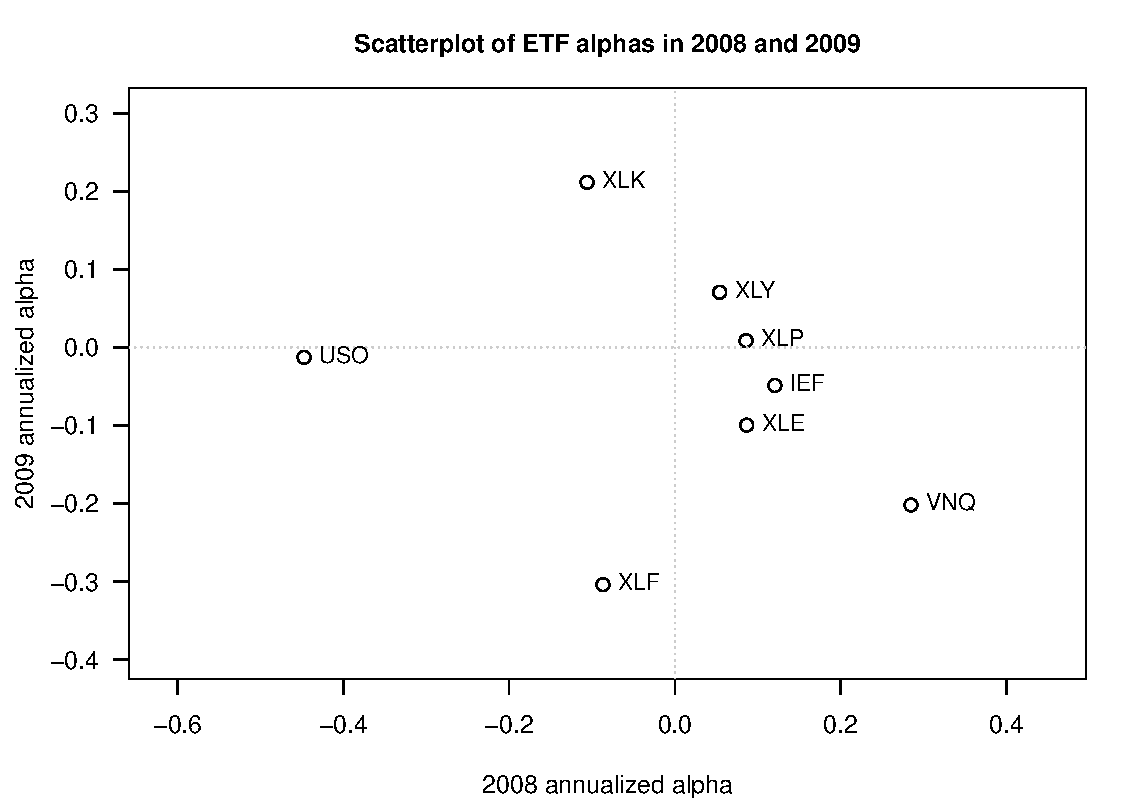
\includegraphics[width=0.95\linewidth]{figures/scatter_etfs.pdf}
\caption{ETF annualized alpha in 2008 versus 2009, using the requested
endpoint intervals and VTI benchmark.}
\label{fig:scatter}
\end{figure}

\smallinput{scatter_alphas_2008_2009.tex}{The eight pairs of annualized
alphas used in Figure~\ref{fig:scatter}.}{tab:scatter}

The cross-sectional Pearson correlation is $\HWAlphaCorrelation$,
indicating weak negative association among these eight points. VNQ changes
from positive to negative alpha, while XLK changes from negative to positive.
XLY and XLP remain positive; USO and XLF remain negative. Overall,
\HWAlphaSignSameCount{} ETFs retain their alpha sign and
\HWAlphaSignChangedCount{} change sign.

The plot supplies little evidence of positive alpha persistence from 2008 to
2009 in this small ETF cross-section. Eight related assets over one pair of
years cannot establish that alpha generally has no relationship across time.
No predictive conclusion or statistical significance claim is inferred from
this figure alone.

\section{Verification and reproducible deliverables}
The supplied sample output is a useful check, but numerical agreement alone
does not establish a correct implementation. The repository's
\texttt{hw1\_results/verify\_hw1.R} performs ten checks, including:
\begin{itemize}
\item reconstructing cumulative bootstrap returns by summing underlying
daily log returns;
\item comparing all horizon allocations with an independent moment-based
optimum, using weights proportional to $\widehat\Sigma^{-1}\widehat\mu$
and checking the long-only bounds;
\item testing the risk function on separate synthetic inputs;
\item fitting ordinary regressions directly with \texttt{lm.fit()} to
verify every year's intercept, beta, and annualized alpha;
\item checking the annual ticker permutations, descending alpha order,
matrix dimensions, and generated PNG artifacts.
\end{itemize}

All ten checks pass. The largest five-horizon allocation difference from the
independent mathematical optimum is approximately $1.62\times10^{-5}$.
The largest annualized-alpha difference before display rounding is
approximately $4.98\times10^{-5}$, within the four-decimal table precision.
The full verification record is reproduced in Appendix~\ref{app:verification}.

The package includes the original assignment and reference images, the
completed submission, this PDF and its LaTeX source, vector and raster
figures, full scenario and annual-statistics exports, the console record,
verification code, setup instructions, and environment/data manifests.
The 1,000 individual scenario values are provided in machine-readable files
alongside this report rather than printed as thousands of table rows.

From the repository root on Windows, run:
\begin{lstlisting}[numbers=none]
Rscript --vanilla setup.R
powershell -ExecutionPolicy Bypass -File build.ps1
\end{lstlisting}
The README gives equivalent R and LaTeX commands for other platforms. The
setup installs missing packages and records the pinned course-package source
commits; it does not silently replace existing installations.

\begin{thebibliography}{9}
\bibitem{univariate} J. Pawlowski. \emph{Univariate Investment Strategies},
FRE7241 course slides, January 20, 2026, especially slides 14--19.
\bibitem{functions} J. Pawlowski. \emph{Functions}, FRE7241 course slides,
January 20, 2026, especially slides 31--40.
\bibitem{dates} J. Pawlowski. \emph{Date and Time Series Objects}, FRE7241
course slides, January 20, 2026, especially the xts indexing and endpoint
sections.
\bibitem{data} J. Pawlowski. \emph{Data Management} and
\emph{Multivariate Time Series}, FRE7241 course slides, CAPM-table examples.
\bibitem{packages} \texttt{rutils} 0.2 and \texttt{PerformanceAnalytics}
2.1.0, installed package implementations and data. Exact GitHub source commits
are recorded in \texttt{reproducibility/package-versions.csv}.
\end{thebibliography}

\clearpage
\appendix
\section{Additional scenario and interval outputs}
\label{app:additional}
\wideinput{short_returns_first5.tex}{First five paired scenarios at the
shortest holding block, $h=596$.}{tab:shortreturns}
\smallinput{short_wealth_first5.tex}{First five optimized portfolio-metric
values at the shortest holding block.}{tab:shortwealth}
\wideinput{bootstrap_overlap.tex}{Historical-window overlap diagnostics.
These describe reuse of historical return intervals, not an effective sample
size estimate.}{tab:overlap}
\wideinput{annual_windows.tex}{All CAPM endpoint intervals, including
their shared boundaries and observation counts.}{tab:windows}
\wideinput{last_window_head.tex}{First six rows of the final endpoint
interval. Values are daily log returns.}{tab:lasthead}
\wideinput{last_window_tail.tex}{Last six rows of the final endpoint
interval. Values are daily log returns.}{tab:lasttail}

\clearpage
\section{Complete annual CAPM tables}
\label{app:capm}
The first interval's complete table appears in Table~\ref{tab:capmfirst}.
The following tables give all remaining intervals. The reported 2012 VNQ
robust downside-beta estimate is subject to the convergence warning described
in the main text. All ordinary-regression outputs used for alpha extraction
were independently verified.
\wideinput{capm_2007.tex}{Complete CAPM statistics for 2007.}{tab:capm2007}
\wideinput{capm_2008.tex}{Complete CAPM statistics for 2008.}{tab:capm2008}
\wideinput{capm_2009.tex}{Complete CAPM statistics for 2009.}{tab:capm2009}
\wideinput{capm_2010.tex}{Complete CAPM statistics for 2010.}{tab:capm2010}
\wideinput{capm_2011.tex}{Complete CAPM statistics for 2011.}{tab:capm2011}
\wideinput{capm_2012.tex}{Complete CAPM statistics for 2012. VNQ robust downside beta is subject to the recorded convergence warning.}{tab:capm2012}
\wideinput{capm_2013.tex}{Complete CAPM statistics for 2013.}{tab:capm2013}
\wideinput{capm_2014.tex}{Complete CAPM statistics for 2014.}{tab:capm2014}
\wideinput{capm_2015.tex}{Complete CAPM statistics for 2015.}{tab:capm2015}
\wideinput{capm_2016.tex}{Complete CAPM statistics for 2016.}{tab:capm2016}
\wideinput{capm_2017.tex}{Complete CAPM statistics for 2017.}{tab:capm2017}
\wideinput{capm_2018.tex}{Complete CAPM statistics for 2018.}{tab:capm2018}
\wideinput{capm_2019.tex}{Complete CAPM statistics for 2019.}{tab:capm2019}
\wideinput{capm_2020.tex}{Complete CAPM statistics for 2020.}{tab:capm2020}
\wideinput{capm_2021.tex}{Complete CAPM statistics for 2021.}{tab:capm2021}
\wideinput{capm_2022.tex}{Complete CAPM statistics for 2022.}{tab:capm2022}
\wideinput{capm_2023.tex}{Complete CAPM statistics for 2023.}{tab:capm2023}
\wideinput{capm_2024.tex}{Complete CAPM statistics for 2024.}{tab:capm2024}
\wideinput{capm_2025.tex}{Complete CAPM statistics for 2025.}{tab:capm2025}
\wideinput{capm_2026.tex}{Complete CAPM statistics for 2026, based on the partial final endpoint interval.}{tab:capm2026}


\clearpage
\section{Complete submitted R code}
\label{app:code}
This is the complete file submitted for the homework, including the original
question comments, diagnostic expressions, and filled-in solutions.
\lstinputlisting{../Panagiotis_Housos_hw1.R}

\clearpage
\section{Complete assignment execution output}
\label{app:execution}
This record contains the outputs of the assignment's diagnostic expressions.
Full additional scenario data and every annual CAPM table are also supplied
in the accompanying CSV/RDS exports.
\lstinputlisting[language={},numbers=none,basicstyle=\ttfamily\tiny,
  xleftmargin=0pt,framexleftmargin=0pt]{../hw1_results/execution_output.txt}

\clearpage
\section{Independent verification record}
\label{app:verification}
\lstinputlisting[language={},numbers=none,basicstyle=\ttfamily\footnotesize,
  xleftmargin=0pt,framexleftmargin=0pt]{../hw1_results/verification.txt}
\end{document}
